% ===========================================================================
% Diagrammi del progetto KeyItaly, disegnati con TikZ.
% Gli stili condivisi sono definiti in preambolo.tex.
% ===========================================================================

% Entità dello schema concettuale: intestazione e, sotto la riga, gli attributi.
\newcommand{\boxEntita}[2]{%
  \begin{tabular}{@{}c@{}}
    \textbf{#1}\\[1.5pt]
    \hline
    \rule{0pt}{2.6ex}%
    \begin{tabular}{@{}l@{}}#2\end{tabular}
  \end{tabular}}

% ---------------------------------------------------------------------------
% Diagramma navigazionale
% ---------------------------------------------------------------------------
\newcommand{\diagrammaNavigazionale}{%
\begin{tikzpicture}[x=1cm, y=1cm, every node/.append style={font=\small}]

  \node[pubblico] (home) at (8,0) {Home};

  \node[pubblico] (carrello)  at ( 0,-2) {Carrello};
  \node[pubblico] (categorie) at ( 4,-2) {Categorie\\catalogo};
  \node[pubblico] (catalogo)  at ( 8,-2) {Catalogo};
  \node[pubblico] (accesso)   at (12,-2) {Login /\\Registrazione};
  \node[admin]    (listaord)  at (16,-2) {Lista ordini};

  \draw[linea] (home.south) -- (8,-1.15);
  \draw[linea] (0,-1.15) -- (16,-1.15);
  \foreach \x in {0,4,8,12,16} { \draw[linea] (\x,-1.15) -- (\x,-1.65); }

  % Carrello
  \node[utente] (checkout)  at (0,-3.8) {Checkout};
  \node[utente] (riepilogo) at (0,-5.5) {Riepilogo\\ordine};
  \draw[linea] (carrello.south) -- (checkout.north);
  \draw[linea] (checkout.south) -- (riepilogo.north);

  % Categorie del catalogo
  \node[pubblico] at (5.3,-3.8) {Tastiere};
  \node[pubblico] at (5.3,-5.3) {Switch};
  \node[pubblico] at (5.3,-6.8) {Copritasti};
  \draw[linea] (categorie.south) -- (4,-6.8);
  \foreach \y in {-3.8,-5.3,-6.8} { \draw[linea] (4,\y) -- (4.25,\y); }

  % Catalogo
  \node[pubblico] at (9.3,-3.8) {Descrizione\\prodotto};
  \node[admin]    at (9.3,-5.3) {Cancella\\prodotto};
  \node[admin]    at (9.3,-6.8) {Aggiungi\\prodotto};
  \node[admin]    at (9.3,-8.3) {Modifica\\prodotto};
  \draw[linea] (catalogo.south) -- (8,-8.3);
  \foreach \y in {-3.8,-5.3,-6.8,-8.3} { \draw[linea] (8,\y) -- (8.25,\y); }

  % Accesso e profilo
  \node[utente] (profilo) at (12,-3.8) {Profilo};
  \draw[linea] (accesso.south) -- (profilo.north);
  \node[utente] at (13.3,-5.5)  {Modifica\\indirizzo};
  \node[utente] at (13.3,-7.1)  {Modifica metodo\\pagamento};
  \node[utente] at (13.3,-8.7)  {Mostra dettagli\\ordine};
  \node[utente] at (13.3,-10.3) {Stampa fattura\\ordine};
  \draw[linea] (profilo.south) -- (12,-10.3);
  \foreach \y in {-5.5,-7.1,-8.7,-10.3} { \draw[linea] (12,\y) -- (12.25,\y); }

  % Legenda
  \begin{scope}[shift={(0,-12.1)}]
    \node[pubblico, minimum height=5mm, text width=17mm] at (0,0)   {pubblico};
    \node[utente,   minimum height=5mm, text width=25mm] at (3.1,0) {utente registrato};
    \node[admin,    minimum height=5mm, text width=25mm] at (6.6,0) {amministratore};
  \end{scope}
\end{tikzpicture}}

% ---------------------------------------------------------------------------
% Mappa dei contenuti
% ---------------------------------------------------------------------------
\newcommand{\mappaContenuti}{%
\begin{tikzpicture}[x=1cm, y=1cm, every node/.append style={font=\small}]

  \node[pubblico] (home) at (7.5,0) {Home};

  \node[pubblico] (carrello)   at ( 0,-2.4)   {Carrello};
  \node[pubblico] (tastiere)   at ( 2.7,-2.4) {Tastiere};
  \node[pubblico] (switchp)    at ( 5.4,-2.4) {Switch};
  \node[pubblico] (copritasti) at ( 8.1,-2.4) {Copritasti};
  \node[utente]   (profilo)    at (11.0,-2.4) {Profilo};
  \node[admin]    (listaord)   at (14.5,-2.4) {Lista ordini};

  \foreach \n in {carrello,tastiere,switchp,copritasti,profilo,listaord}
    { \draw[freccia] (home) to[out=-90,in=90] (\n); }

  \node[utente]   (checkout)  at ( 0,-4.8)   {Checkout};
  \node[pubblico] (prodotto)  at ( 5.4,-4.8) {Prodotto};
  \node[utente]   (indirizzo) at ( 9.6,-4.8) {Indirizzo};
  \node[utente]   (pagamento) at (12.7,-4.8) {Metodo di\\pagamento};
  \node[utente]   (storico)   at (11.0,-7.1) {Storico\\ordini};
  \node[utente]   (ordine)    at ( 9.6,-9.4) {Ordine};
  \node[utente]   (fattura)   at (12.7,-9.4) {Fattura};

  \draw[freccia] (carrello) -- (checkout);
  \foreach \n in {tastiere,switchp,copritasti}
    { \draw[freccia] (\n) to[out=-90,in=90] (prodotto); }
  \draw[freccia] (profilo) to[out=-90,in=90] (indirizzo);
  \draw[freccia] (profilo) to[out=-90,in=90] (pagamento);
  \draw[freccia] (profilo) -- (storico);
  \draw[freccia] (storico) to[out=-90,in=90] (ordine);
  \draw[freccia] (ordine) -- (fattura);
  % L'amministratore raggiunge lo stesso dettaglio d'ordine dalla lista completa
  \draw[freccia] (listaord.south) -- (14.5,-10.7) -- (9.6,-10.7) -- (ordine.south);
\end{tikzpicture}}

% ---------------------------------------------------------------------------
% Schema concettuale della base di dati
% ---------------------------------------------------------------------------
\newcommand{\schemaER}{%
\begin{tikzpicture}[x=1cm, y=1cm,
    ent/.style={draw=black, line width=.6pt, fill=white, rounded corners=1pt,
                inner sep=5pt, font=\scriptsize, align=center},
    rel/.style={draw=black, line width=.6pt, fill=white, diamond, aspect=3.2,
                inner sep=1pt, minimum width=2.9cm, font=\scriptsize, align=center},
    card/.style={font=\scriptsize, inner sep=2pt, fill=white}]

  % --- Utente e specializzazioni ---
  \node[ent] (utente) at (6,0) {\boxEntita{Utente}{%
      \underline{username}\\ password\\ nome, cognome\\ email \textit{(unico)}\\ data di nascita}};

  \node[ent] (cliente) at (2.6,-4.6) {\boxEntita{Cliente}{%
      \textit{metodo di pagamento:}\\
      \quad nome, cognome carta\\
      \quad numero, scadenza, CVV\\[2pt]
      \textit{indirizzo di fatturazione:}\\
      \quad via, CAP, città}};

  \node[ent] (admin) at (9.6,-4.6) {\boxEntita{Admin}{\textit{nessun attributo}\\ \textit{proprio}}};

  \draw[line width=.6pt] (cliente.north) -- (2.6,-3.0) -- (9.6,-3.0) -- (admin.north);
  \draw[line width=.6pt] (6,-3.0) -- (6,-2.3);
  \draw[-{Triangle[length=5pt,width=7pt]}, line width=.9pt] (6,-2.6) -- (utente.south);
  \node[font=\scriptsize, anchor=west] at (6.25,-2.75) {generalizzazione};

  % --- Ordini ---
  \node[rel] (esecuzione) at (2.6,-7.6) {Esecuzione};
  \draw[line width=.6pt] (cliente.south) -- (esecuzione.north);
  \node[card, anchor=west] at (2.7,-6.9) {(0,N)};

  \node[ent] (ordine) at (2.6,-10.8) {\boxEntita{Ordine}{%
      \underline{ID}\\ prezzo totale\\ data ordine, data consegna\\
      destinatario: nome, cognome\\ consegna: via, CAP, città}};
  \draw[line width=.6pt] (esecuzione.south) -- (ordine.north);
  \node[card, anchor=west] at (2.7,-8.5) {(1,1)};

  % --- Acquisti ---
  \node[rel] (acquisto) at (7.6,-10.8) {Acquisto};
  \draw[line width=.6pt] (ordine.east) -- (acquisto.west);
  \node[card, anchor=south] at (5.5,-10.7) {(1,N)};
  \node[ent, draw=black!55, dash pattern=on 2pt off 1.5pt] (attrAcq) at (7.6,-8.6)
    {\begin{tabular}{@{}l@{}}quantità\\ prezzo di acquisto\\ IVA di acquisto\end{tabular}};
  \draw[line width=.5pt, draw=black!55, dash pattern=on 2pt off 1.5pt]
    (acquisto.north) -- (attrAcq.south);

  \node[ent] (prodotto) at (12.3,-10.8) {\boxEntita{Prodotto}{%
      \underline{ID}\\ nome, descrizione\\ prezzo, IVA\\ grafica\\ quantità in stock}};
  \draw[line width=.6pt] (acquisto.east) -- (prodotto.west);
  \node[card, anchor=south] at (10.0,-10.7) {(0,N)};

  % --- Specializzazioni del prodotto ---
  \node[ent] (tastiere)   at ( 9.0,-14.4) {Tastiere};
  \node[ent] (switchp)    at (12.3,-14.4) {Switch};
  \node[ent] (copritasti) at (15.4,-14.4) {Copritasti};
  \draw[line width=.6pt] (tastiere.north) -- (9.0,-13.5) -- (15.4,-13.5) -- (copritasti.north);
  \draw[line width=.6pt] (switchp.north) -- (12.3,-13.5);
  \draw[-{Triangle[length=5pt,width=7pt]}, line width=.9pt] (12.3,-13.5) -- (prodotto.south);
\end{tikzpicture}}

% ---------------------------------------------------------------------------
% Wireframe della pagina principale
% ---------------------------------------------------------------------------
\newcommand{\wireframeHome}{%
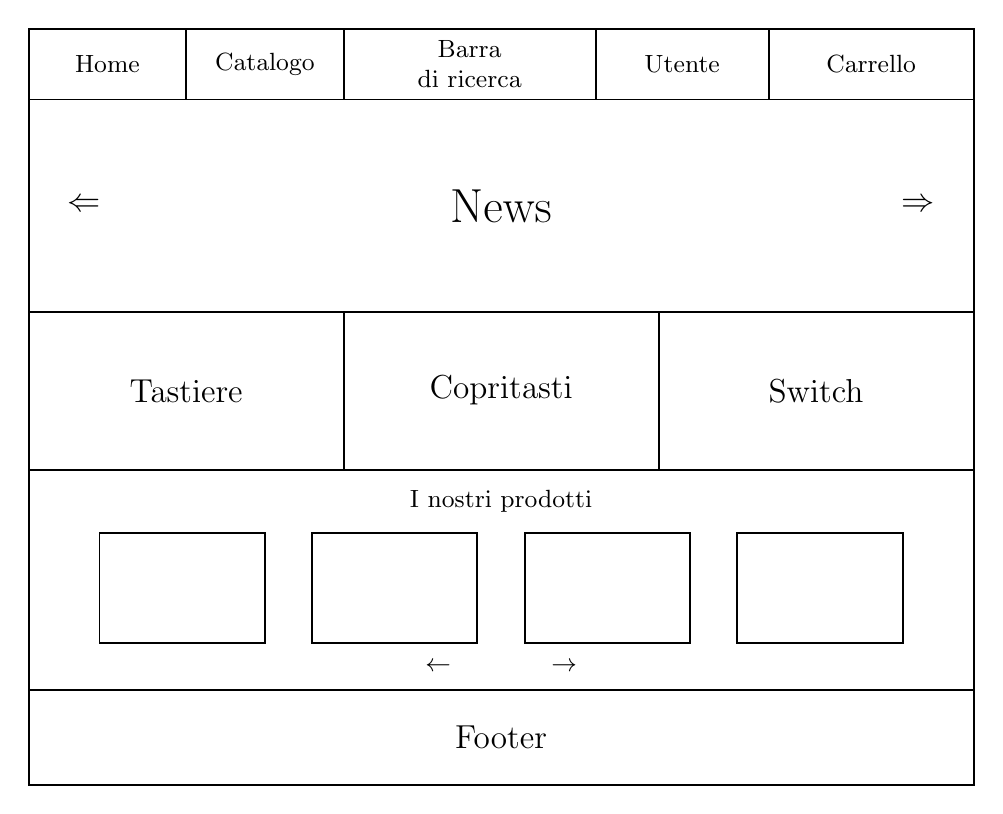
\begin{tikzpicture}[x=1cm, y=1cm,
    riquadro/.style={draw=black, line width=.7pt, align=center}]

  \def\W{12}

  \draw[riquadro] (0,0) rectangle (\W,-0.9);
  \foreach \x in {2,4,7.2,9.4} { \draw[line width=.7pt] (\x,0) -- (\x,-0.9); }
  \node[font=\small] at (1,-0.45) {Home};
  \node[font=\small] at (3,-0.45) {Catalogo};
  \node[font=\small, align=center] at (5.6,-0.45) {Barra\\di ricerca};
  \node[font=\small] at (8.3,-0.45) {Utente};
  \node[font=\small] at (10.7,-0.45) {Carrello};

  \draw[riquadro] (0,-0.9) rectangle (\W,-3.6);
  \node[font=\LARGE] at (6,-2.25) {News};
  \node[font=\large] at (0.7,-2.25) {$\Leftarrow$};
  \node[font=\large] at (11.3,-2.25) {$\Rightarrow$};

  \draw[riquadro] (0,-3.6) rectangle (\W,-5.6);
  \foreach \x in {4,8} { \draw[line width=.7pt] (\x,-3.6) -- (\x,-5.6); }
  \node[font=\large] at (2,-4.6)  {Tastiere};
  \node[font=\large] at (6,-4.6)  {Copritasti};
  \node[font=\large] at (10,-4.6) {Switch};

  \draw[riquadro] (0,-5.6) rectangle (\W,-8.4);
  \node[font=\small] at (6,-6.0) {I nostri prodotti};
  \foreach \x in {0.9,3.6,6.3,9.0}
    { \draw[line width=.7pt] (\x,-6.4) rectangle ++(2.1,-1.4); }
  \node[font=\small] at (5.2,-8.1) {$\leftarrow$};
  \node[font=\small] at (6.8,-8.1) {$\rightarrow$};

  \draw[riquadro] (0,-8.4) rectangle (\W,-9.6);
  \node[font=\large] at (6,-9.0) {Footer};
\end{tikzpicture}}

% ---------------------------------------------------------------------------
% Palette cromatica
% ---------------------------------------------------------------------------
\newcommand{\paletteColori}{%
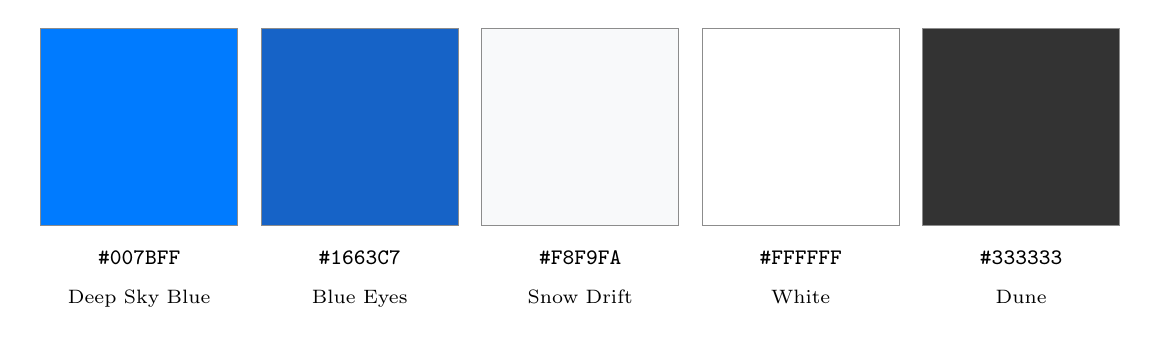
\begin{tikzpicture}[x=1mm,y=1mm]
  \definecolor{deepskyblue}{HTML}{007BFF}
  \definecolor{blueeyes}{HTML}{1663C7}
  \definecolor{snowdrift}{HTML}{F8F9FA}
  \definecolor{dune}{HTML}{333333}

  \foreach \i/\col/\hex/\nome in {
    0/deepskyblue/007BFF/Deep Sky Blue,
    1/blueeyes/1663C7/Blue Eyes,
    2/snowdrift/F8F9FA/Snow Drift,
    3/white/FFFFFF/White,
    4/dune/333333/Dune}
  {
    \fill[\col,draw=black!45] (\i*28,0) rectangle ++(25,25);
    \node[anchor=north,font=\footnotesize\ttfamily] at (\i*28+12.5,-2) {\#\hex};
    \node[anchor=north,font=\scriptsize,text width=26mm,align=center]
      at (\i*28+12.5,-7) {\nome};
  }
\end{tikzpicture}}

% ---------------------------------------------------------------------------

% ---------------------------------------------------------------------------
% Mappa delle servlet, dei filtri e delle viste
% ---------------------------------------------------------------------------
\newcommand{\mappaServlet}{%
\begin{tikzpicture}[x=1cm, y=1cm,
    srv/.style={nodo, fill=cUtente, text width=40mm, font=\footnotesize\ttfamily},
    jsp/.style={nodo, fill=cVista,  text width=40mm, font=\footnotesize\ttfamily},
    esito/.style={nodo, fill=cAdmin, text width=40mm, font=\footnotesize},
    tit/.style={font=\small\bfseries, anchor=west},
    flt/.style={font=\footnotesize, anchor=west}]

  % ======================= Area pubblica =======================
  \node[tit] at (-2.2,1.2) {Area pubblica};

  \node[srv] (r1) at (0,0)      {/};
  \node[jsp] (v1) at (5.4,0)    {home.jsp};

  \node[srv] (r2) at (0,-1.9)   {/Catalogo\\/Tipo};
  \node[jsp] (v2) at (5.4,-1.9) {catalogo.jsp\\catalogoAdmin.jsp};

  \node[srv] (r3) at (0,-3.9)   {/DescrizioneProdotto};
  \node[jsp] (v3) at (5.4,-3.9) {descrizione.jsp};

  \node[srv] (r4) at (0,-6.1)   {/Login\\/Logout\\/Registrazione};
  \node[jsp] (v4) at (5.4,-6.1) {login.jsp};

  \node[srv] (r5) at (0,-8.3)   {/AggiungiProdotto\\/RimuoviProdotto};
  \node[jsp] (v5) at (5.4,-8.3) {carrello.jsp};

  \node[srv] (r6) at (0,-10.6)    {/ajax/search\\/CheckEmail\\/api/GetImage};
  \node[esito] (v6) at (5.4,-10.6) {risposte JSON\\e immagini del catalogo};

  \foreach \a/\b in {r1/v1, r2/v2, r3/v3, r4/v4, r5/v5, r6/v6}
    { \draw[freccia] (\a) -- (\b); }

  % ======================= Area /user/* =======================
  \node[tit] at (11.3,1.2) {Riservata a \texttt{/user/*}};

  \node[srv] (u1) at (13.5,-0.2) {/user/Profilo\\/user/ModificaIndirizzo\\/user/ModificaPagamento};
  \node[jsp] (w1) at (18.9,-0.2) {profilo.jsp};

  \node[srv] (u3) at (13.5,-2.6) {/user/Checkout};
  \node[jsp] (w3) at (18.9,-2.6) {checkout.jsp};
  \node[jsp] (w4) at (18.9,-4.0) {acquisto.jsp};

  \node[srv] (u4) at (13.5,-5.5)   {/user/StampaFattura};
  \node[esito] (w5) at (18.9,-5.5) {fattura in PDF};

  \draw[freccia] (u1) -- (w1);
  \draw[freccia] (u3) -- (w3);
  \draw[freccia] (w3) -- (w4);
  \draw[freccia] (u4) -- (w5);

  \node[draw=cBordo, dash pattern=on 3pt off 2pt, rounded corners=3pt,
        fit=(u1)(w1)(u4)(w5), inner sep=7pt] (boxuser) {};
  \node[flt] at (11.3,-7.0) {protetta da \texttt{UserFilter}};

  % ======================= Area /admin/* =======================
  \node[tit] at (11.3,-8.4) {Riservata a \texttt{/admin/*}};

  \node[srv] (a1) at (13.5,-9.6) {/admin/OrdiniAdmin};
  \node[jsp] (x1) at (18.9,-9.6) {ordiniAdmin.jsp};

  \node[srv] (a2) at (13.5,-11.1) {/admin/ModificaProdotto};
  \node[jsp] (x2) at (18.9,-11.1) {modifica.jsp};

  \node[srv] (a3) at (13.5,-12.9) {/admin/SaveProdotto\\/admin/DeleteProdotto};
  \node[jsp] (x3) at (18.9,-12.9) {catalogoAdmin.jsp};

  \foreach \a/\b in {a1/x1, a2/x2, a3/x3} { \draw[freccia] (\a) -- (\b); }

  \node[draw=cBordo, dash pattern=on 3pt off 2pt, rounded corners=3pt,
        fit=(a1)(x1)(a3)(x3), inner sep=7pt] (boxadmin) {};
  \node[flt] at (11.3,-14.4) {protetta da \texttt{AdminFilter}};

  % ======================= Filtro sulle viste =======================
  \node[srv, fill=cFiltro] (jspf) at (0,-12.5) {JspFilter};
  \node[esito] (forbidden) at (5.4,-12.5) {403 Forbidden};
  \draw[freccia] (jspf) -- (forbidden);
  \node[font=\footnotesize, text width=80mm, align=center] at (2.7,-13.9)
    {ogni accesso diretto a \texttt{/pages/views/*}};

\end{tikzpicture}}
